\chapter{Prototypos de interfaz}
En este capítulo adjunte y describa los prototipos de la interfaz para su aplicación. Procure hacer referencia al diseño de interacción y diseño para la usabilidad presentes en su aplicación.
Si su aplicación tiene propiedades de accesibilidad para un público con necesidades especiales, por favor describa las estrategias usadas en esta sección.

\section{Prototipos de la funcionalidad X}
Recuerde poner un texto introductorio breve para cada sección.
\vspace{2cm}
\begin{figure}[H]
  \centering
    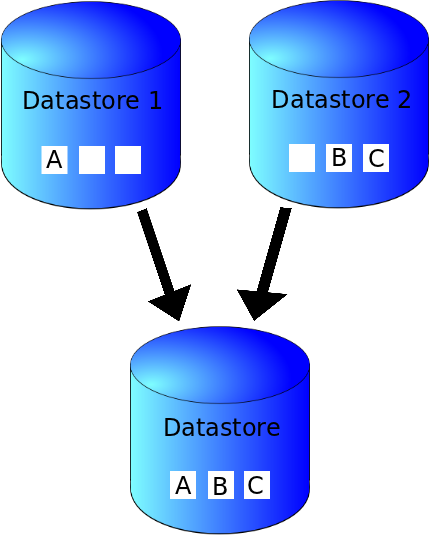
\includegraphics[height= 11cm, width=17cm]{project/images/data-sync}
\end{figure}
\newpage
\begin{figure}[H]
  \centering
    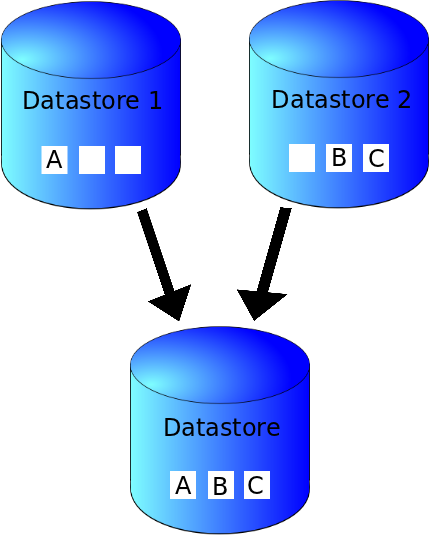
\includegraphics[height= 11cm, width=17cm]{project/images/data-sync}
\end{figure}
\vspace{1cm}

\section{Prototipos de la funcionalidad Y}
No olvide referenciar las imágenes en el texto usando \emph{label} y \emph{ref}.

\begin{figure}[H]
  \centering
    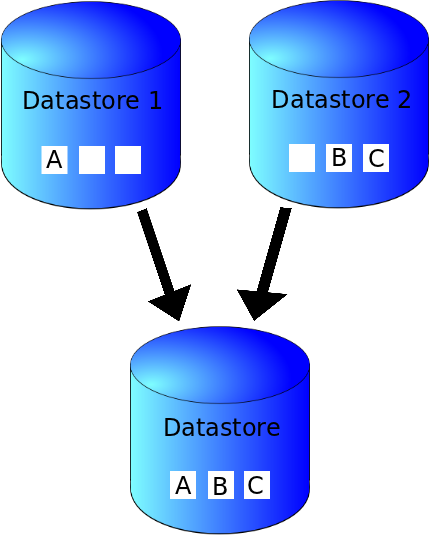
\includegraphics[height= 11cm, width=17cm]{project/images/data-sync}
\end{figure}